\chapter{Loop Closures using an Omni Camera}
\label{chapter:omni_loop_close}

\section{Place Recognition}

The first step is to substitute omni camera images in the place recognition module. The donut image format is not preferred for the place recognition.  It has blind spots (inner and outer circle), which contain some texture, and are also susceptible to change from internal reflections within the lense.  In terms of place recognition, this would add noise to each image and therefore the unwrapped image is preferred.

Therefore unwrapped circular images are used for place recognition.  The exact details of unwrapping and associating omni camera frames with stereo frames is discussed in Section \ref{sec:video_input}.

As described in section \ref{sec:bag_of_words}, the place recognition system employs clustering of detected SURF features in feature space using a bag of words approach.  This means that in the case of $360^\circ$ circular images, the bag of words representation will be invariant to rotations about the omni camera frame z axis (Fig \ref{fig:omni_coord_sys}), as the locations of 2D features are not considered.  This is ideal for this particular use case.

\section{Loop closures}
\label{sec:calc_loop_edge}

A match from the place recognition module itself is not enough to do a global loop closure.  As described in section \ref{sec:scavislam_place_recog}, a geometry check is required to filter false positive matches and determine a metric rigid body transformation so the loop closure may be added to the graph.

It has also been mentioned in section \ref{subsec:selected_approach} that calculating a transformation using a monocular camera such as the omni camera introduces the arbitrary scale issue.  (For further explanation of the scale issue, see Chapter \ref{chapter:MultiCamSLAM}). Therefore the stereo data needs to be associated with the omni camera data in order to produce a metric scale transformation.  Two methods were developed and compared to address this scale issue.  The first approach uses the p3p algorithm and is a fairly straightforward algorthm.  The second ``scale correction algorithm is a more sophisticated approach.  These methods will be discussed in detail and compared in the following sections. 

\subsection{Circular Matching}

%TODO circular matching citation
%TODO siftgpu citation

For both approaches, there is a data association stage between omni camera images and stereo images.  Features were extracted from stereo images and the unwrapped spherical image using SIFTGPU.  Matching is then performed, also using SIFTGPU between left and right, left and omni and right and omni.  These three match lists are filtered for robust matches using circular matching. 

\begin{figure}[h]
  \centering
    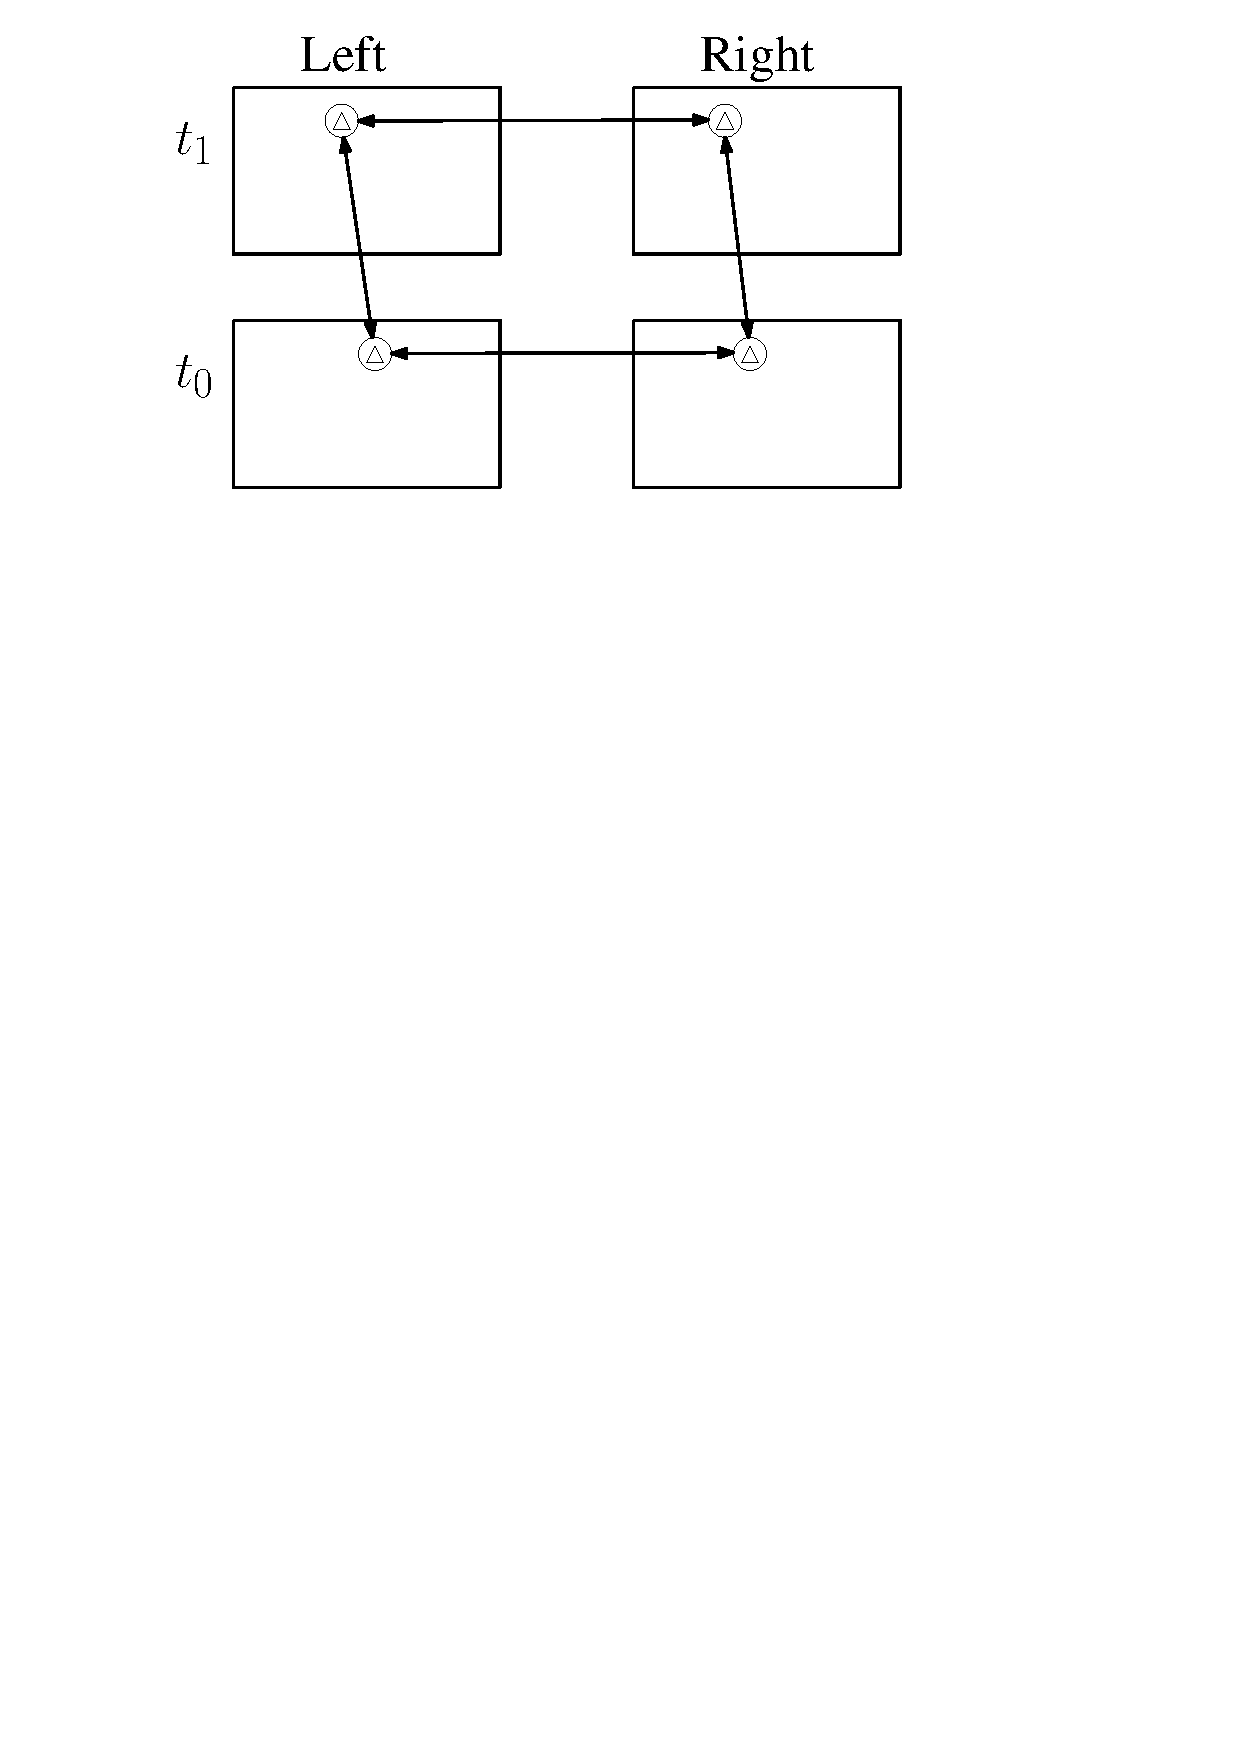
\includegraphics[width=0.5\textwidth]{chapters/images/stereo_circular_matching}\\
  \caption{Circular matching for two pairs of stereo frames at $t_0$ and $t_1$. A feature must match across all frames to be accepted}
  \label{fig:stereo_circular_matching}
\end{figure}

Fig. \ref{fig:stereo_circular_matching} shows an example of stereo matching applied to two stereo image pairs.  The idea behind circular matching is to create a chain of matches across multiple frames, whereby the chain forms a closed loop of matches. 

The basic algorithm for circular matching is as follows:  
\begin{itemize} \itemsep1pt  \parskip0pt \parsep0pt
 \item Take a feature in the first frame.  
 \item Look up its match in the next frame.  
 \item Take this match and look up its match in the next frame.  
 \item Continue for all frames
 \item Check to see if last feature also has a match with the feature from the first frame.  
 \subitem If so then accept the match.
\end{itemize}

Circular matching is very efficient, as it only involves iteration of match lists and lookups of matches.  It provides much more robust matching, which means that the SIFT match threshold may be relaxed, allowing the possibility for more correct matches. An example of circular matching can be found in Fig. \ref{fig:circular_match} 

\begin{figure}[h]
  \centering
    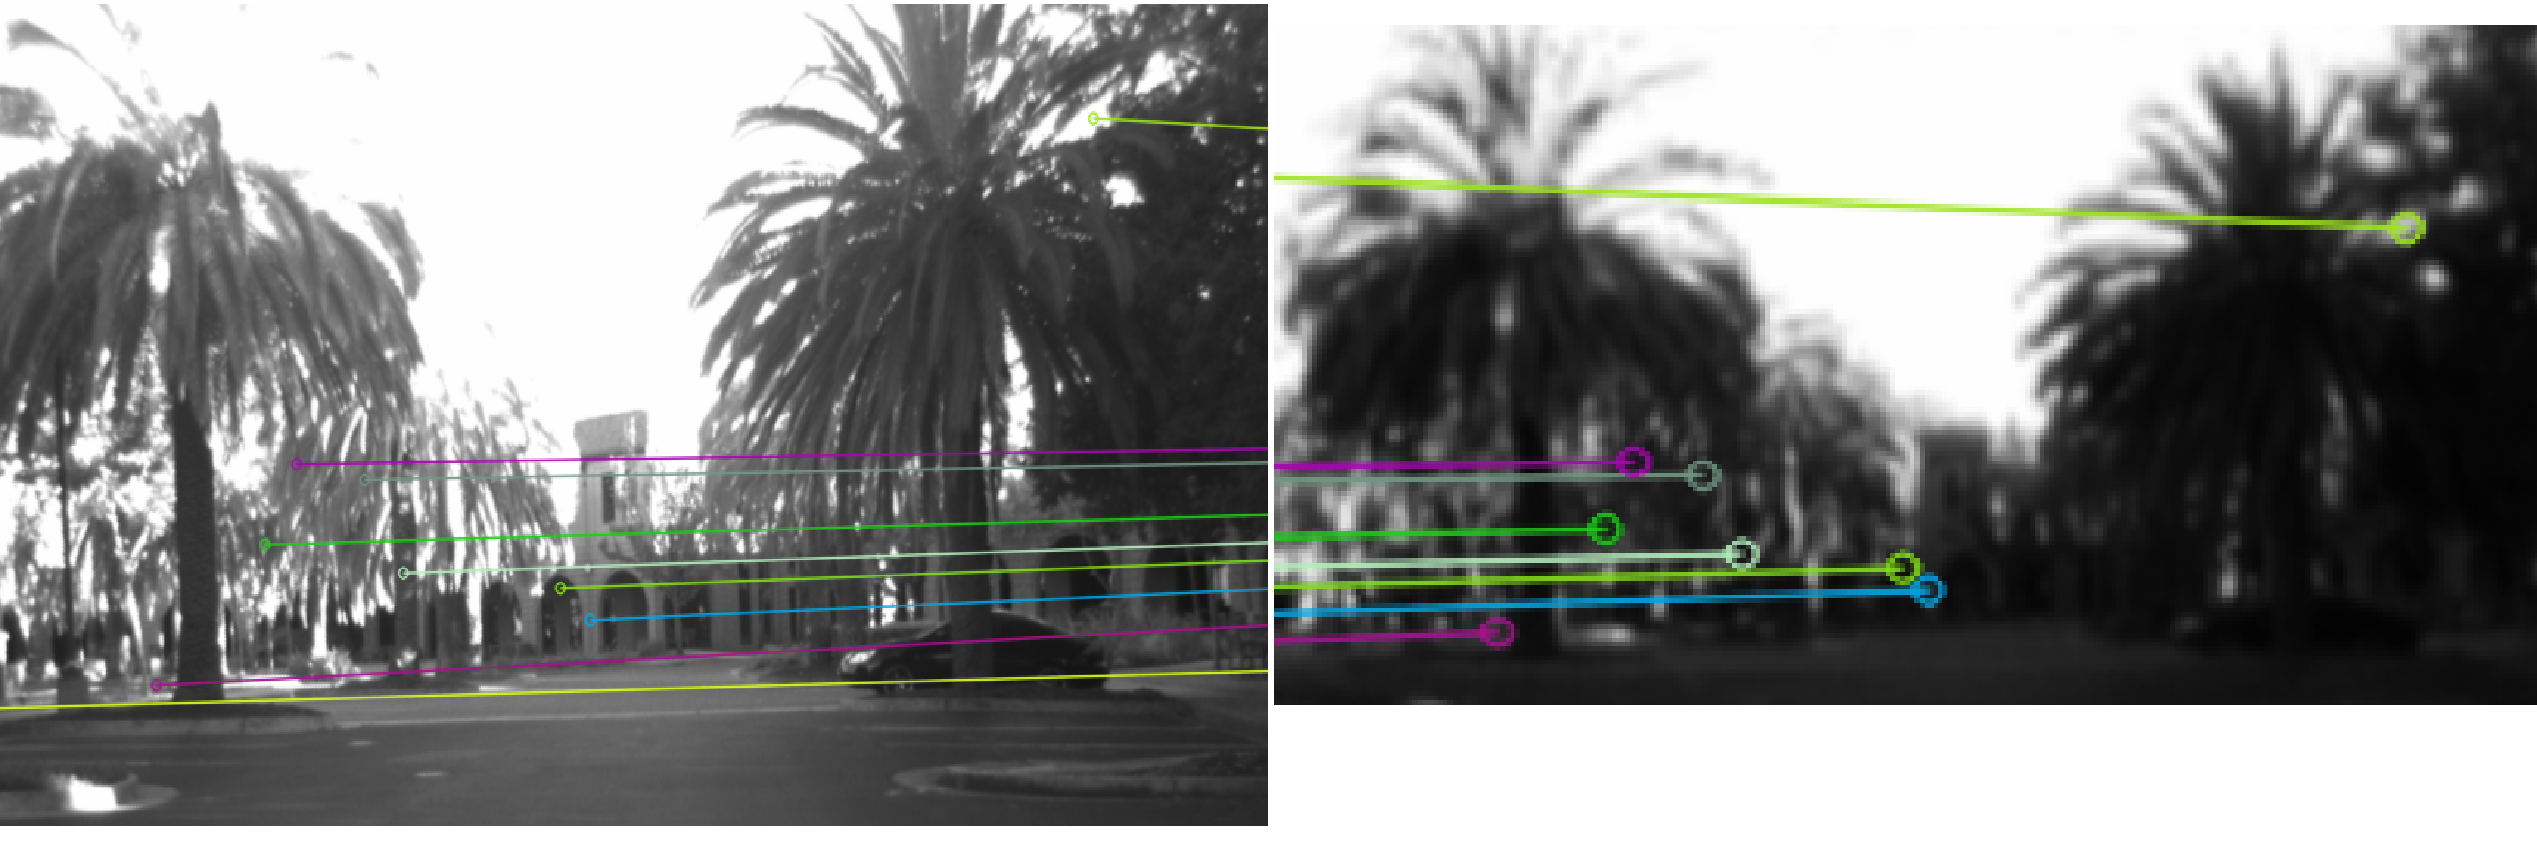
\includegraphics[width=1.0\textwidth]{chapters/images/circular_match}\\
  \caption{Results of circular matching between left, right and omni frames. Left is one of the stereo images and right is a cropped part of the unwrapped omni image. The circular matching produces robust matches without having strict SIFT matching thresholds}
  \label{fig:circular_match}
\end{figure}

\subsection{p3p Algorithm}

%As opposed to the two step approach described above, this implementation calculates a metric transformation using stereo and omni camera data in one step.

The p3p algorithm (Section \ref{subsec:p3p}) calculates a transformation between frames given a set of 2D to 3D correspondences.  The scale of the transformation is propagated from the 3D points.  This means that after triangulating the new 2D points with the transformation obtained, they will be to the same scale as the existing map.

The pipeline implemented using the p3p algorithm is as follows:

\begin{enumerate}
\itemsep0em
 \item Perform circular matching between left/right images from one keyframe, and omni image from the other keyframe
 \item Triangulate 3D points in metric scale using left/right stereo circular matches
 \item Use p3p algorithm; correspondences are known between 3D stereo points and 2D omni points
\end{enumerate}

\begin{figure}[h]
  \centering
    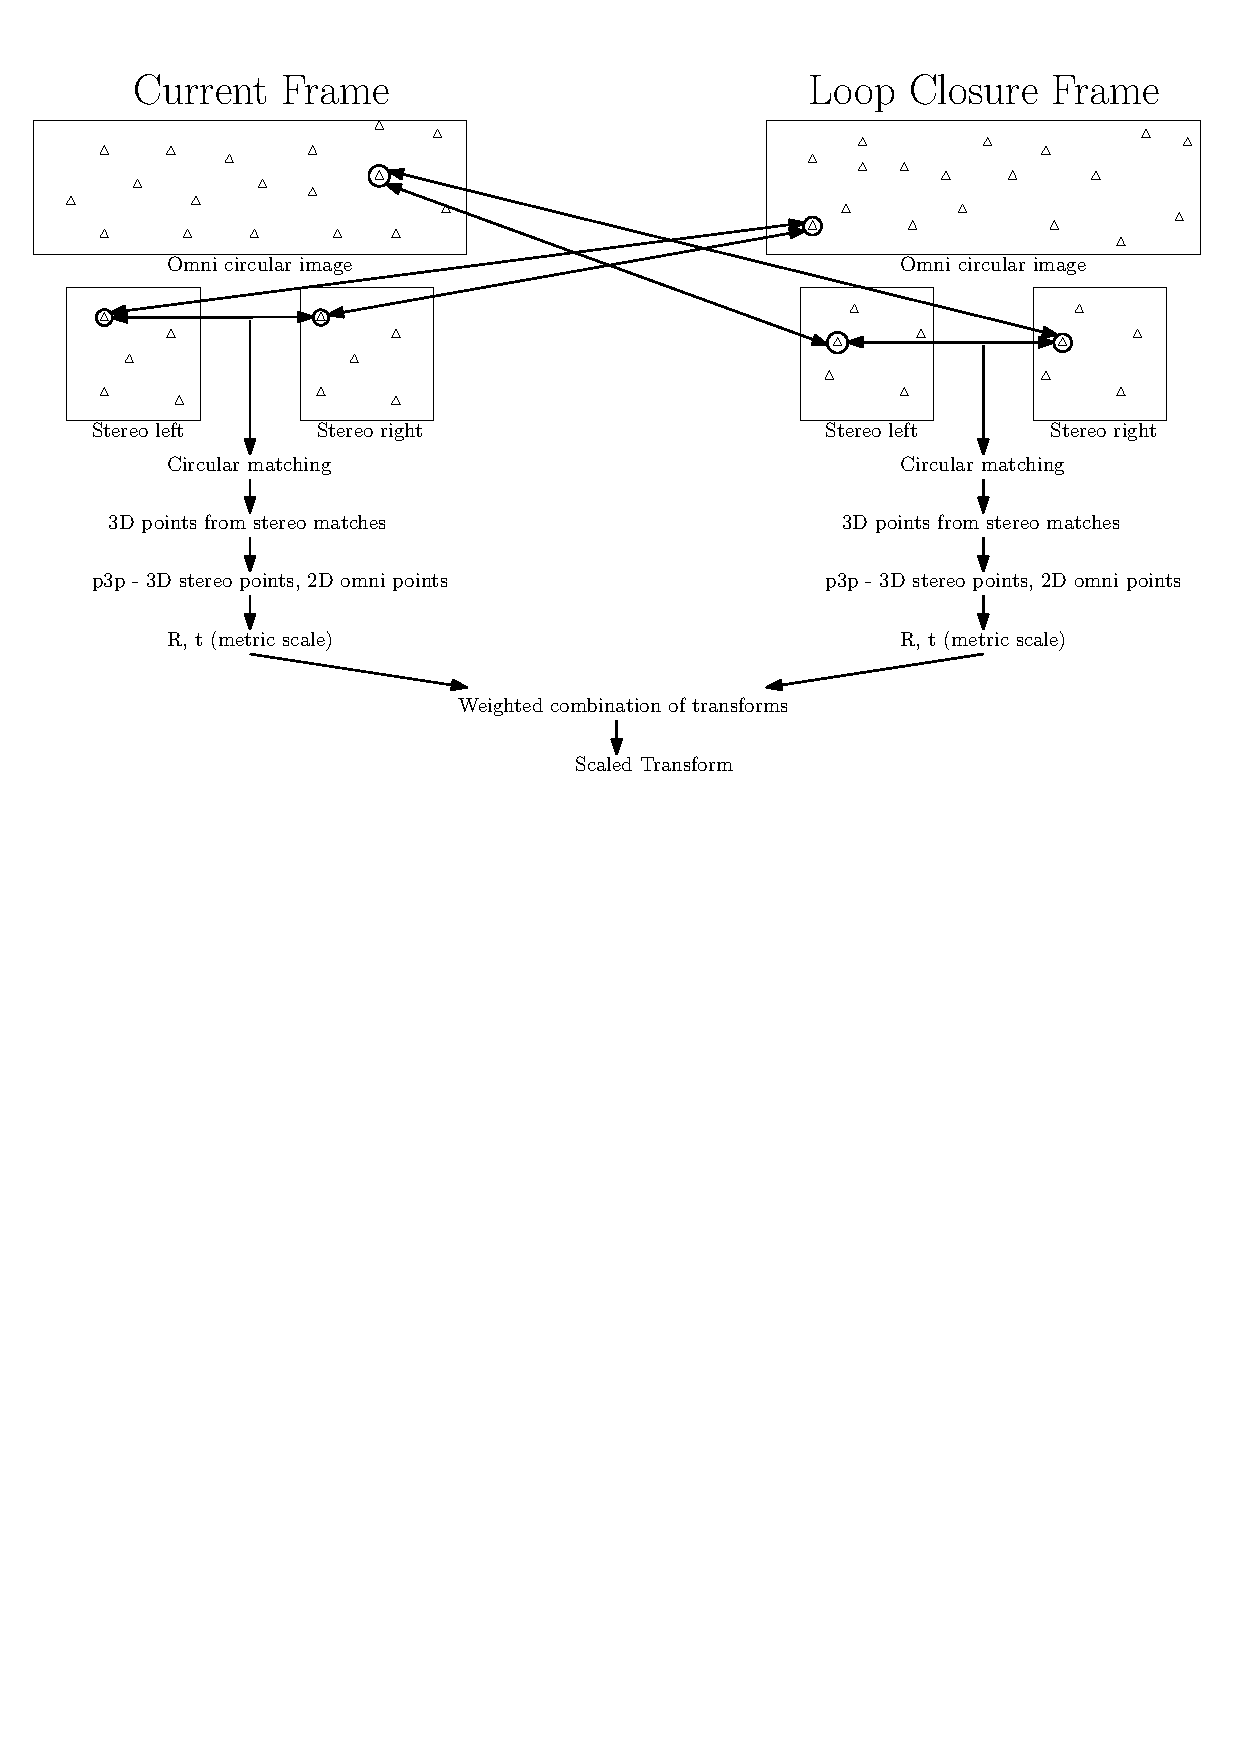
\includegraphics[width=1.0\textwidth]{chapters/images/6_images_p3p}\\
  \caption{Outline of the p3p based pipeline}
  \label{fig:p3p_flowchart}
\end{figure}

This is also illustrated in Fig. \ref{fig:p3p_flowchart}.  This will directly calculate a pose between the two keyframes to the correct scale.  It can also be run twice, matching stereo and omni in both directions, returning two transformations. In terms of implementation this is a straightforward solution, and would be preferred.  

\subsection{Scale Correction algorithm}

This algorithm is a two stage approach: Firstly, calculate the non-metric transformation using images from the omni camera, and then correct it to metric scale using stereo data.  An important consideration is that the omni camera will find loop closures where stereo would not, so one must assume that there will be likely zero overlap between stereo poses, and therefore no feature matching possible between these two frames. Fig. \ref{fig:omni_loop_close}

\subsubsection{Pose estimation}

The first step is to calculate a non metric transformation using the two omni frames only.  This is done using the 5 point algorithm as mentioned in Section \ref{subsec:5point} paired with RANSAC and evaluating euclidean distance as the error function.  This step could have been improved by adding a non linear refinement step calculating a refined pose based on all inlier points.  The algorithm returns a non metric pose and a set of inlier points, represented as 3D vectors (also non metric scale).

\subsubsection{Scale Offset Calculation}

Points with metric scale are calculated using matches between left and right stereo frames.  These points are then matched to feature points from the omni camera images and compared with 3D non metric points returned from the pose estimation.  A scale offset is calculated per point as follows:

\begin{align}
  \centering
  %\begin{align}
   S =
   \displaystyle\frac{
   \left|\displaystyle\frac{ {M}_{x}}{ P_{x}}\right| + 
   \left|\displaystyle\frac{ {M}_{y}}{ P_{y}}\right| + 
   \left|\displaystyle\frac{ {M}_{z}}{ P_{z}}\right|
   }
   {3}
  %\end{align}
  \label{eq:scale_offset}
\end{align}

Where $\bv{M}$ is a 3D metric point calculated from stereo, and $\bv{P}$ is a 3D non metric point triangulated based on the pose from the 5 point algorithm.  This formula calculates 3 separate scale offsets from 3 axes and averages them together to one scale offset. 

The pipeline that calculates a list of scale offsets is listed below, and represented in Fig. \ref{fig:scale_adjust_flowchart}.  This pipeline takes left, right and omni images as an input, and may be applied to either of the two loop closure frames separately.  In practice both frames are used and the scale list are concatenated together.

\begin{enumerate}
\itemsep0em
 \item Perform circular matching between left/right/omni images %TODO screenshot
 \item Triangulate 3D points in metric scale using left/right stereo circular matches
 \item For each 3D stereo point:
 \begin{enumerate}
   \item Ensure the matching omni point was an inlier used in pose estimation
   \item Obtain the 3D non metric point triangulated from 5 point transformation
   \item Transform the stereo point to the omni camera frame from the extrinsic calibration $\bv P_{OM} =  ^{OM}\bv T_{ST} \bv P_{ST}$
   \item Calculate scale offset as per formula \ref{eq:scale_offset} %TODO
   \item Add to list of offsets 
 \end{enumerate}
\end{enumerate} 

\begin{figure}[h]
  \centering
    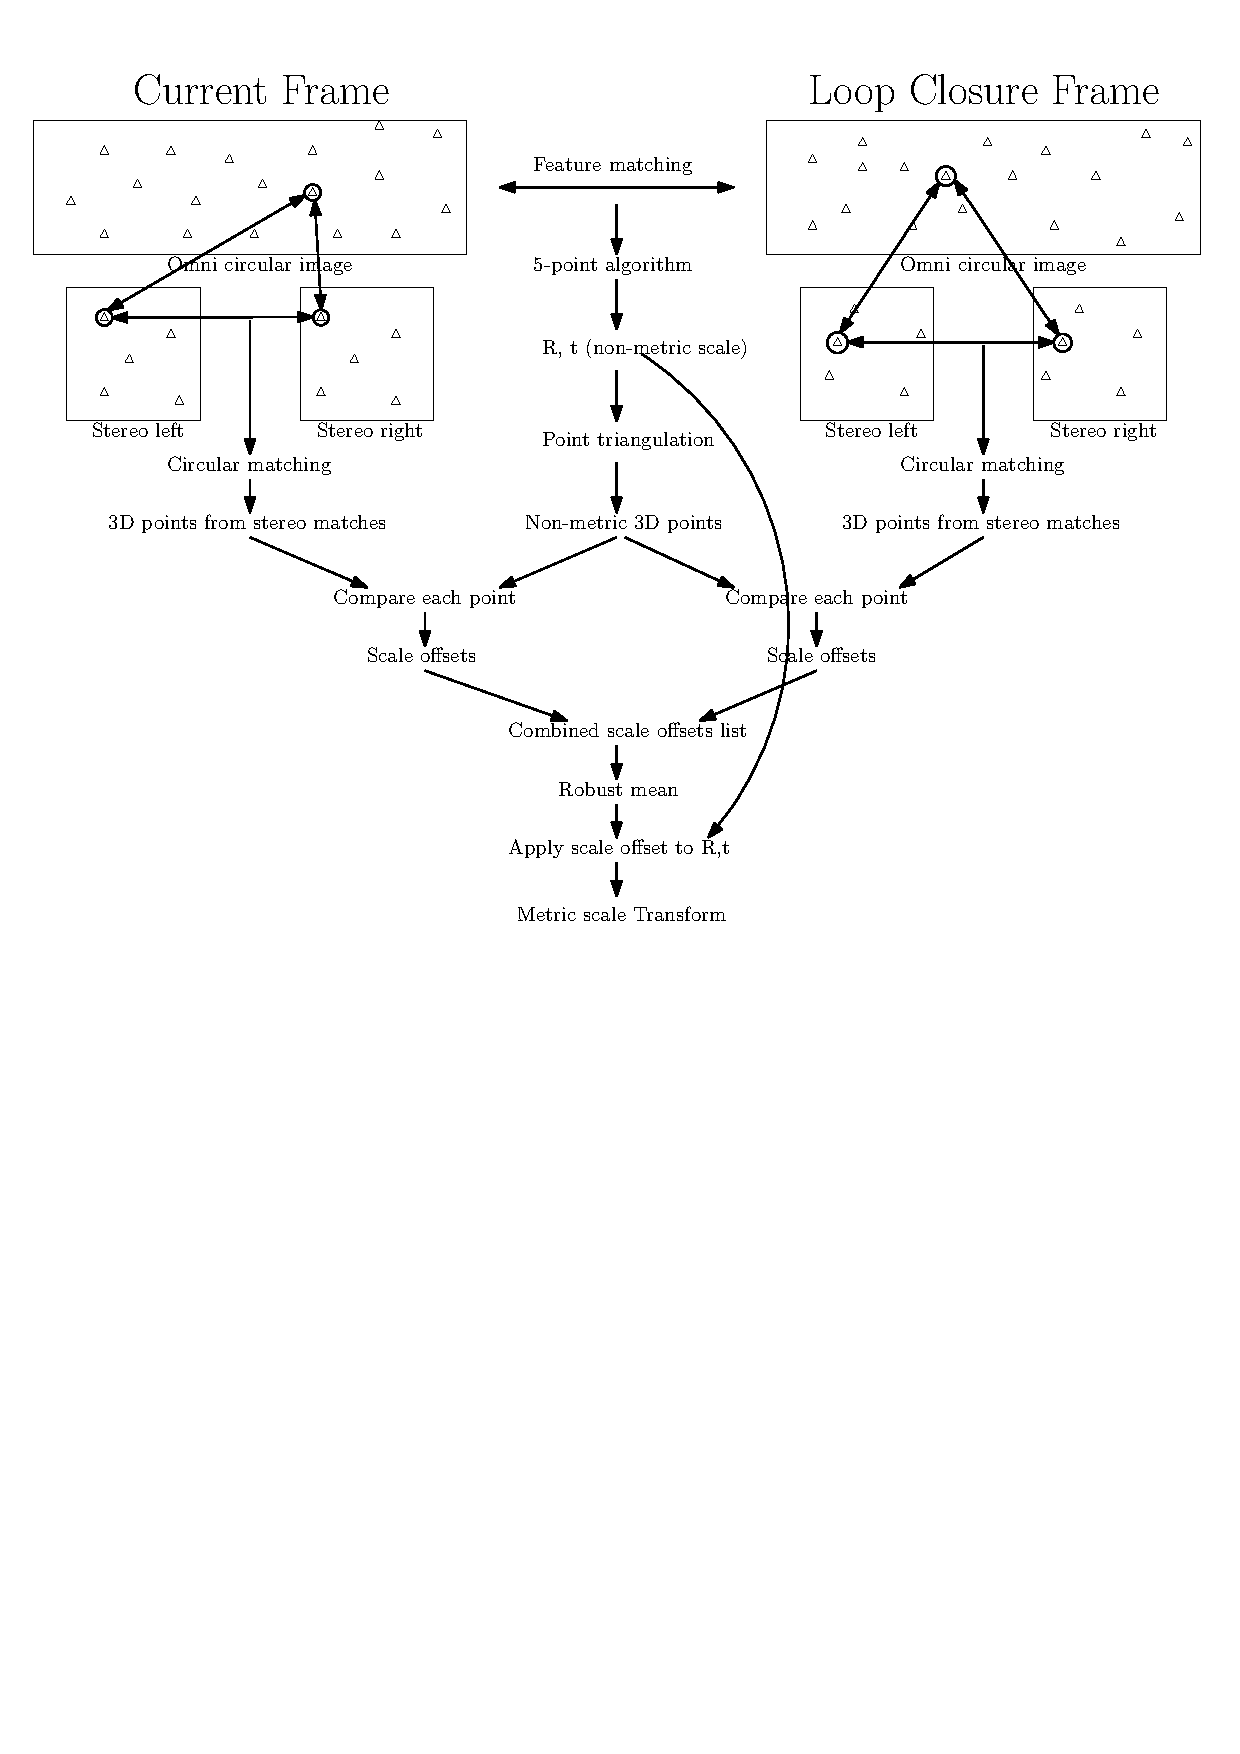
\includegraphics[width=1.0\textwidth]{chapters/images/6_images_scale_adjust}\\
  \caption{Outline of the scale adjustment pipeline}
  \label{fig:scale_adjust_flowchart}
\end{figure}

\subsubsection{Robust scale estimation}

Having determined a number of scale offsets, a single offset needs to be determined.  It is likely that outliers exist in the data and these need to be taken into consideration.  In addition to outliers, it is also important to consider the metric accuracy of each stereo point.  As points occur further away from the camera, the corresponding disparity decreases.  For low values of disparity, the resolution in depth decreases quadratically, and therefore the accuracy of scale estimation from this point diminishes. Fig. \ref{fig:scale_bar_graph} illustrates the relationship between scale offset accuracy and associated depth values.
\begin{figure}[h]
  \centering
    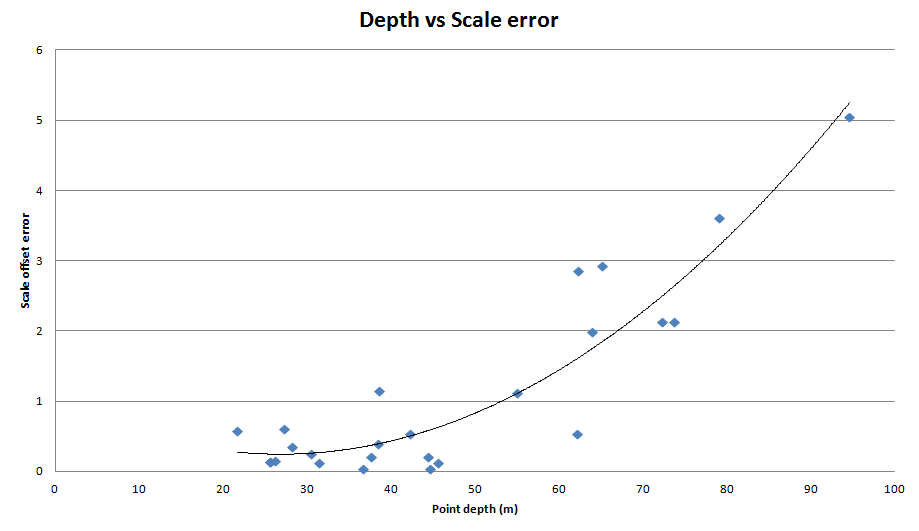
\includegraphics[width=1.0\textwidth]{chapters/images/distance_vs_scale_error}\\
  \caption{Point depth vs scale offset error}
  \label{fig:scale_bar_graph}
\end{figure}

%\begin{figure}[h]
  %\centering
    %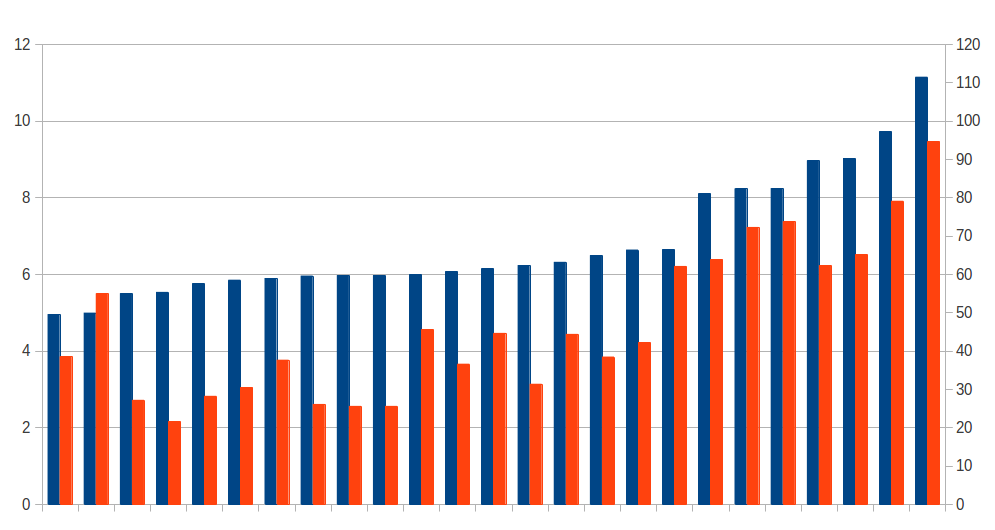
\includegraphics[width=1.0\textwidth]{chapters/images/scale_offset_bar_graph}\\
  %\caption{Scale offsets and corresponding depth values.  The scale offsets are blue with the units on the left and the depth values are orange with the units in meters on the right. In this example the correct scale offset was determined to be 6.11.  From the graph it is clear that scale offsets that differ significantly from the correct offset value are attributed with higher depth values.}
  %\label{fig:scale_bar_graph}
%\end{figure}

It would be possible to apply RANSAC in this case, choosing a random scale offset to scale all of the points and using the sum of euclidean distance between correspondences as an error function.  This would be computationally expensive, and also requires parameter tuning.  So rather a 'weighted mean' strategy was applied, after having explicitly handled the outliers.
%TODO citaion
In order to compensate for outliers, first a robust mean is calculated using (citation) robust mean algorithm.  Outliers can then be identified by comparing them with the robust mean and removed from the list. To deal with the depth uncertainty of points, a weighted average is calculated as follows:

\begin{equation}
\centering
s_{mean} = \dfrac{\displaystyle\sum\limits_{i=0}^n{\dfrac{s_i}{z_i^2}}}
{\displaystyle\sum\limits_{i=0}^n{\dfrac{1}{z_i^2}}}
\end{equation}

$s_i$ denotes a single scale offset, and $z_i$ is the corresponding depth value as calculated by stereo matching.  The idea behind this calculation is to provide weights inversely proportional to the depth of the point, such that distant points are heavily penalised.  Before applying this weighting strategy, the scale calculation was often over estimated and sometimes unstable.  This weighted mean function provided much more stable and accurate scale offsets.

%TODO robust mean citation

%\begin{figure}[h]
  %\centering
    %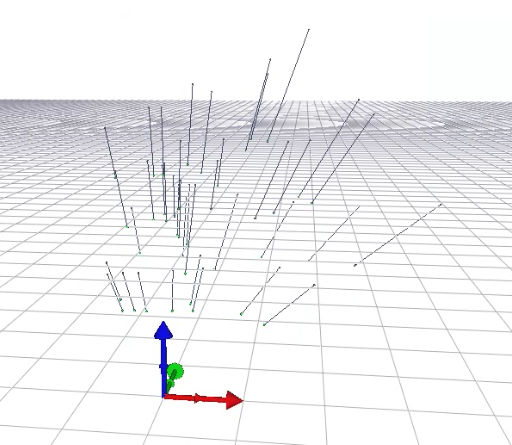
\includegraphics[width=0.6\textwidth]{chapters/images/scale_matches}\\
  %\caption{Visualization of non metric points and their corresponding metric scale matches}
  %\label{fig:circular_match}
%\end{figure}

\subsection{Comparison of approaches}

A number of loop closure examples were evaluated with both the scale correction and p3p approaches, and compared against a ground truth generated by GPS.  Fig. \ref{fig:scale_vs_p3p} shows such an example.  Although both algorithms returned accurate rotations, it is clear that the translation is significantly incorrect for the p3p implementation.

The number of circular matches between the stereo camera and the omni camera of the other keyframe is typically very low.  Not only is matching occuring between different cameras, resulting in differing scale and intensities of feature patches, but there is also a larger translation between cameras. Whilst in the scale correction algorithm, these matches are only used for scale adjustment, in the p3p pipeline they are used for pose estimation.  Scale adjustment only requires one correspondence, however pose estimation requires three.  There are likely to be outliers and therefore desirably a multiple of the minimum number of correspondences is required to determine a good pose.  Therefore the scale correction algorithm should perform better with a limited number of circular matches.

The scale adjustment algorithm uses all the matches between two omni poses to calculate a transformation.  In practice this was found to to be typically well over 100 inliers for pose estimation.  Therefore this results in a highly accurate transformation.  On the other hand, the p3p algorithm only uses the circular matches, which are often as little as 20 matches.  In addition, the rotation part of the transformation calculated by the 5 point algorithm does not need to be scaled, and is unaffected by any inaccuracy in the scale correction part.

\begin{figure}[h]
  \centering
    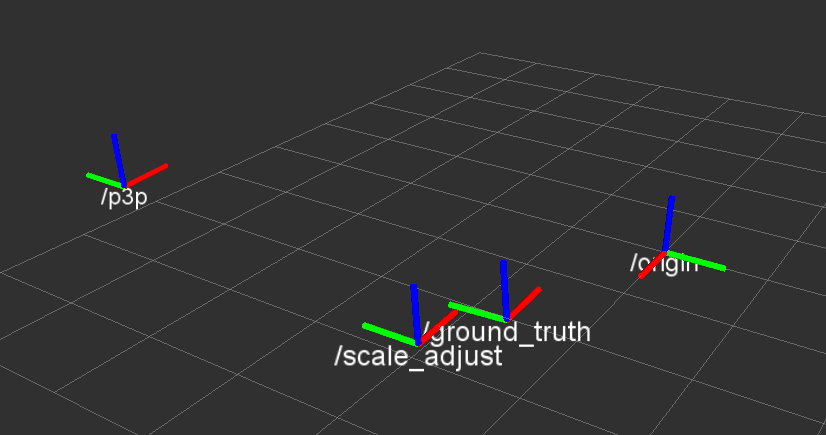
\includegraphics[width=0.9\textwidth]{chapters/images/scale_vs_p3p_1}\\
  \caption{An example comparing pose estimation from p3p and scale adjustment algorithms}
  \label{fig:scale_vs_p3p}
\end{figure}

%TODO: change pic to black on white

Finally another advantage of the scale adjustment algorithm is the way in which the data from both frames is fused.  For both algorithms, they can be run twice by as there are two stereo/omni camera pairs to run the pipeline on. (See Fig. \ref{fig:p3p_flowchart} and Fig. \ref{fig:scale_adjust_flowchart})   Whilst the scale adjustment algorithm outputs two offset vectors that can easily be combined to determine a single robust offset value, the p3p implementation generates two separate poses that need to be fused together somehow.  They could be averaged or both added to the graph weighted on the number of inliers. Nevertheless, incorporating all available data into calculating one transformation should achieve better results than calculating two less accurate poses and averaging them together.

Given this comparison, the scale correction algorithm was selected for use in the omni-loop-closure pipeline to be evaluated.

\begin{figure}[H]
  \centering
    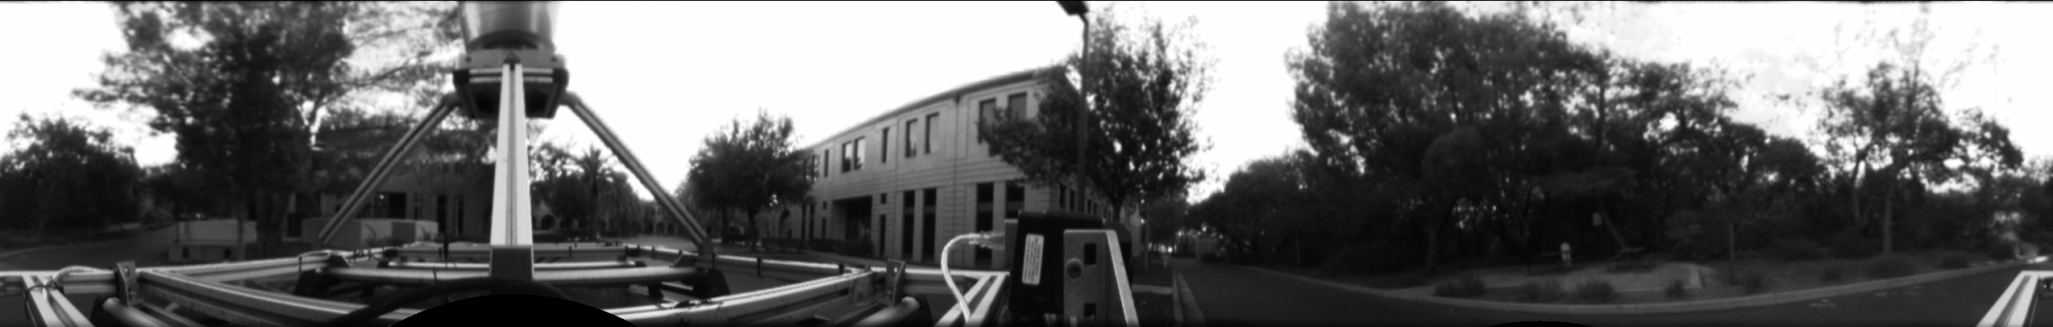
\includegraphics[width=1.0\textwidth]{chapters/images/omni_source}\\
    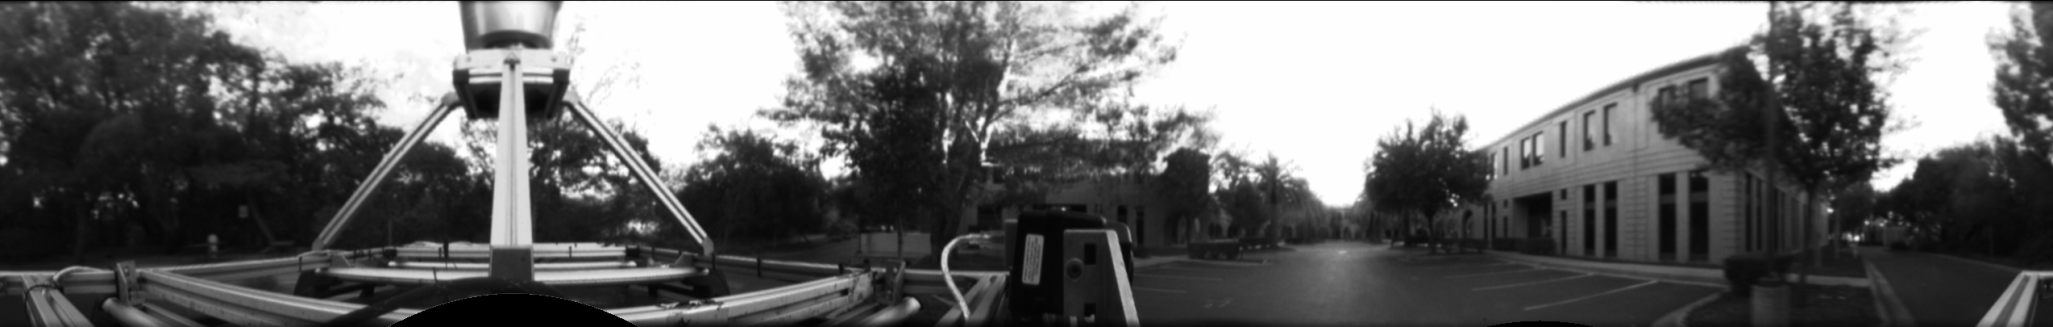
\includegraphics[width=1.0\textwidth]{chapters/images/omni_target}\\
    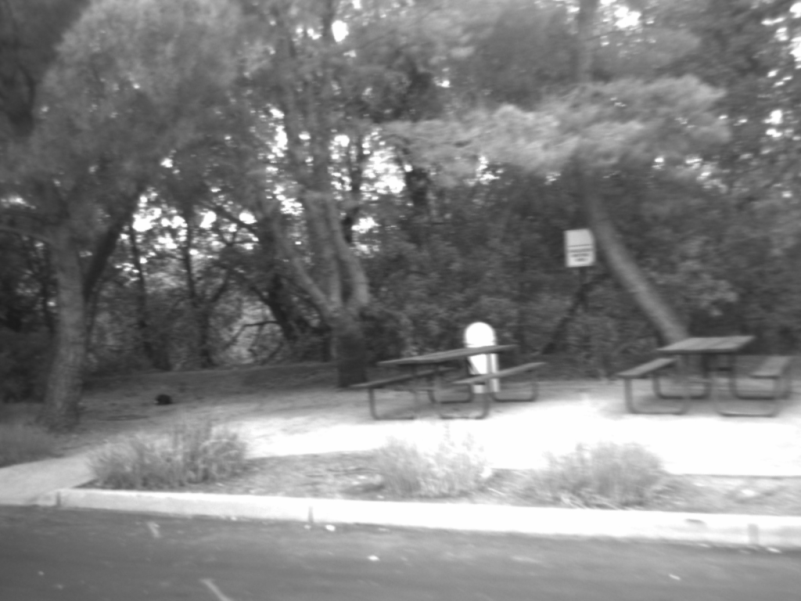
\includegraphics[width=0.49\textwidth]{chapters/images/stereo_source}
    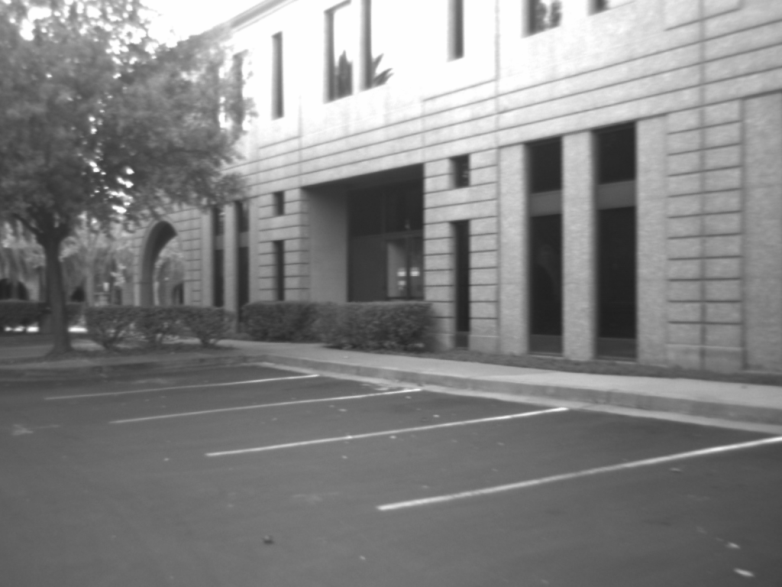
\includegraphics[width=0.49\textwidth]{chapters/images/stereo_target}\\
    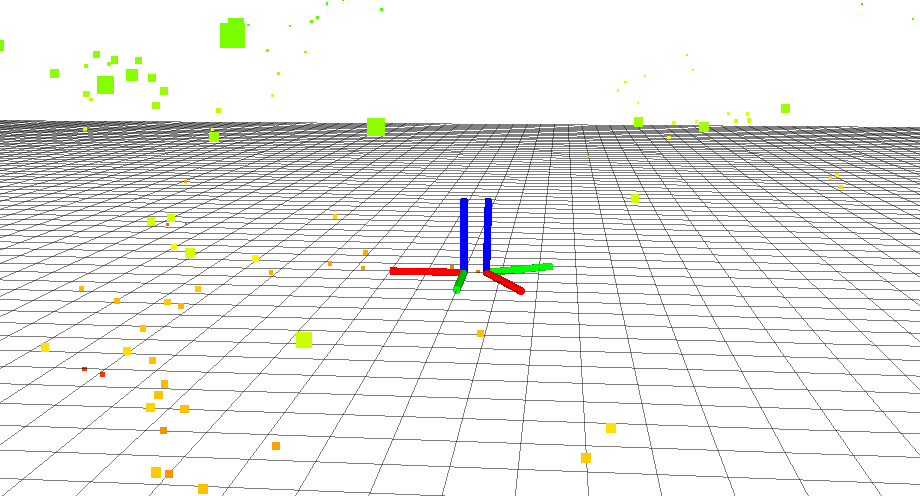
\includegraphics[width=1.0\textwidth]{chapters/images/loop_closure_pose}
  \caption{Example of a pose invariant loop closure using scale adjustment algorithm.  Top shows the two omni images.  Middle shows what the stereo camera sees from these poses.  There is clearly no overlap in the stereo frames.  Bottom shows the metric transformation visualized as a pose, along with 3D pose inlier points in metric scale.}
  \label{fig:}
\end{figure}
\section{Introducing loop closure constraints to the SLAM graph}

Having obtained a transformation between frames, this needs to be integrated into the SLAM graph.  This is not straightforward, especially given that the ScaViSLAM graph utilises the double window approach.  (Sec. \ref{sec:scavislam_graph}).  This section outlines how an edge was added to the graph.

\subsection{Bundle Adjustment vs Pose-Pose edge}

Section \ref{sec:calc_loop_edge} describes returning a single SE(3) edge constraint between keyframes.  This edge can easily be added to the graph.  It would also be just as valid for the pipeline to provide 3D landmarks and shared observations as an output.  In this case the 3D landmarks would be added to the graph as vertices and the shared observations would be added as reprojection edge constraints.  The graph optimization would then calculate the relative pose constraint based on all shared observations, as per a typical bundle adjustment.  The advantage of this is that it more accurately represents the constraint between keyframes than an SE(3) edge  with an estimated information matrix.  In addition, this would work well for the p3p pipeline, as it solves the problem of how to combine two separate transformations.  Using this representation, consecutive loop closures could add even more observations to existing landmarks to further refine the poses.  However, in order to achieve this, the data association for all landmarks would need to be handled.  This essentially means building a whole new SLAM system, which is beyond the scope of this work.

Given that no data association will be done between multiple loop closures, there is little advantage in calculating the constraint using bundle adjustment.  Calculating a keyframe pose-pose edge and estimating the information matrix closely approximates the constraint and is also far more computationally efficient.  Finally, implementing the bundle adjustment, accounting for the double window approach would also be considerably more effort than SE(3) edges.

\subsection{Adding the pose to the inner window}

The place recognition module will return potential loop closures for the most recently added keyframe.  If a loop closure is successful, this means it will connect to a keyframe in the inner window.  However, adding a single edge to the inner window will have little effect, as there will be too many landmark observation constraints opposing this edge.  Typically what happens is that the particular keyframe will be pulled in the direction of the loop closure, but all the other keyframes will remain in place. (fig. \ref{fig:graph_fail})

\begin{figure}[h]
  \centering
    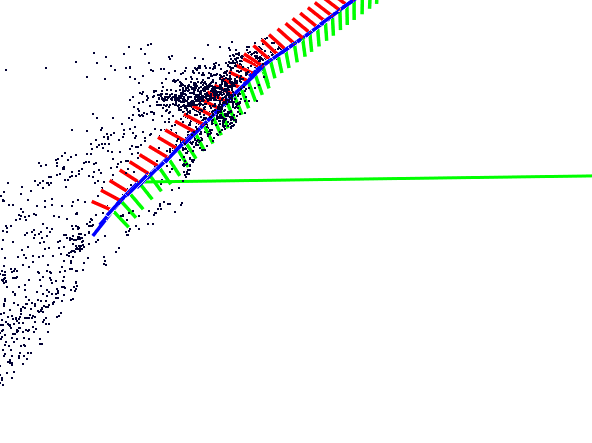
\includegraphics[width=0.49\textwidth]{chapters/images/before_opt}
    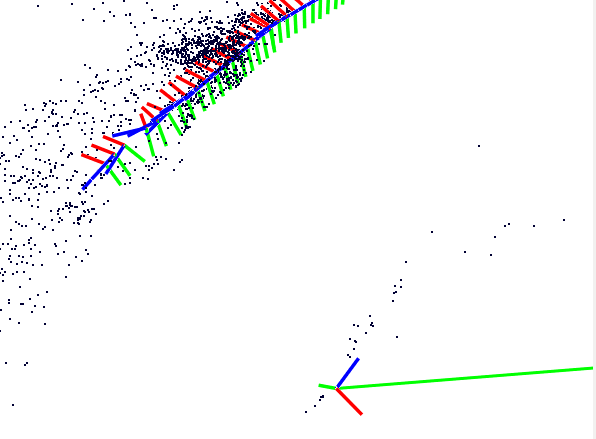
\includegraphics[width=0.49\textwidth]{chapters/images/after_opt}
  \caption{Adding a SE(3) edge to the inner window.  Black dots denote landmarks.  The green line is the SE(3) loop closure edge}
  \label{fig:graph_fail}
\end{figure}

In order to deal with this problem, after adding a loop closure edge, the graph is 'reinitialised' to a new configuration using SE(3) edge only optimization.  The entire inner window is marginalised to SE(3) edges, as they would be when leaving the inner window.  This is essentially the same as changing the inner window size to 1.  Then optimization is performed, this time with the loop closure edge having a more equal weighting to the rest of the constraints.  The graph error is then spread evenly throughout the graph, and the current pose is moved to the loop closure keyframe.  Having completed this optimization, the inner window is restored and the graph retains its structure.

\begin{figure}[h]
  \centering
    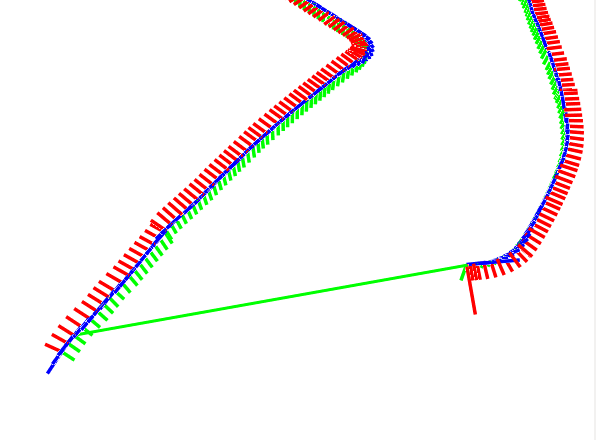
\includegraphics[width=0.45\textwidth]{chapters/images/before_opt_good}
    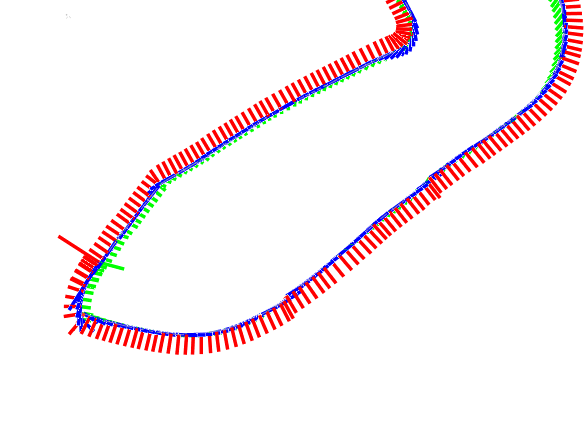
\includegraphics[width=0.45\textwidth]{chapters/images/after_opt_good}
  \caption{Before and after optimization using pose only constraints}
  \label{fig:graph_fail}
\end{figure}